\section{Results}

\begin{figure}[H]
  \centering
  \begin{subfigure}[t]{0.49\linewidth}
    \centering
    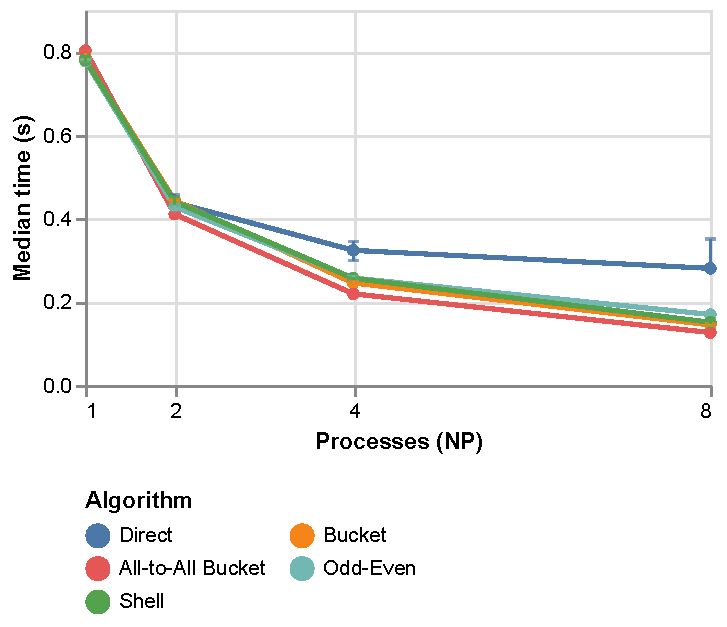
\includegraphics[width=\linewidth]{comparison-time.pdf}
    \caption{Median run time. The error bars show the minimum and the maximum of the 5 runs.}
    \label{fig:comparison-time}
  \end{subfigure}
  \hfill
  \begin{subfigure}[t]{0.49\linewidth}
    \centering
    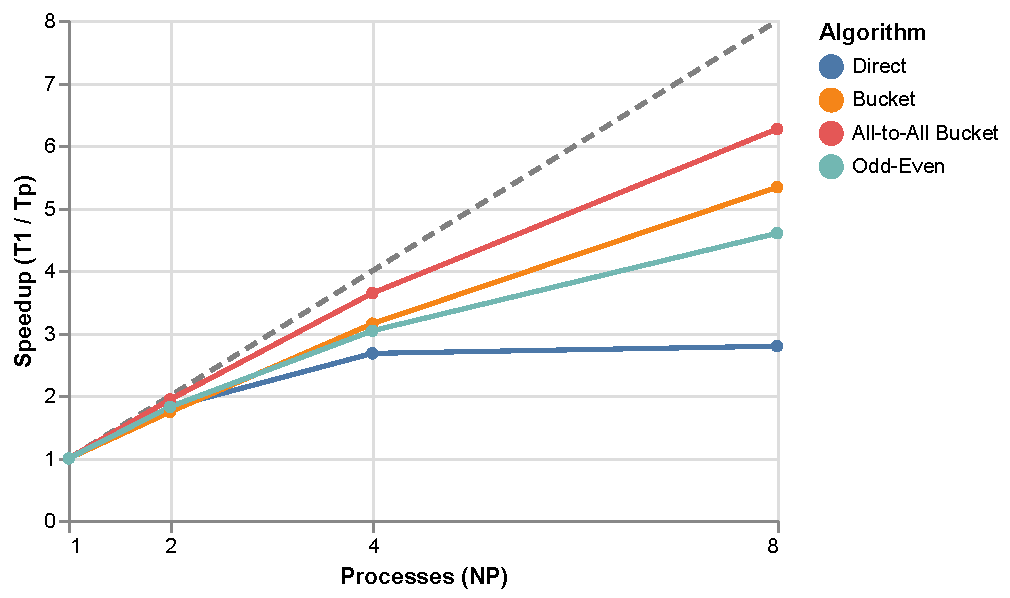
\includegraphics[width=\linewidth]{comparison-speedup.pdf}
    \caption{Speedup. The dashed line shows the ideal speedup.}
    \label{fig:comparison-speedup}
  \end{subfigure}
  \caption{Run time and speedup of all algorithms for $n = 10^7$.}
  \label{fig:comparison}
\end{figure}

\begin{table}[H]
  \centering
  \small
  \setlength{\tabcolsep}{3pt}
  \begin{subtable}[t]{0.49\linewidth}
    \centering
    \begin{tabular}{rrrrr}
  \toprule
  NP & Direct & Bucket & All-to-All & Odd-Even \\
  \midrule
  1 & 0.781 & 0.782 & 0.800 & 0.782 \\
  2 & 0.430 & 0.448 & 0.412 & 0.429 \\
  4 & 0.291 & 0.248 & 0.219 & 0.257 \\
  8 & 0.279 & 0.146 & 0.128 & 0.170 \\
  \bottomrule
\end{tabular}

    \caption{Median run time (s).}
    \label{tab:comparison-time}
  \end{subtable}
  \hfill
  \begin{subtable}[t]{0.49\linewidth}
    \centering
    \begin{tabular}{rrrrr}
  \toprule
  NP & Direct & Bucket & All-to-All Bucket & Odd-Even \\
  \midrule
  1 & 1.00 & 1.00 & 1.00 & 1.00 \\
  2 & 1.82 & 1.74 & 1.94 & 1.83 \\
  4 & 2.68 & 3.16 & 3.64 & 3.04 \\
  8 & 2.80 & 5.34 & 6.27 & 4.60 \\
  \bottomrule
\end{tabular}

    \caption{Speedup.}
    \label{tab:comparison-speedup}
  \end{subtable}
  \caption{Run time and speedup of all algorithms for $n = 10^7$.}
  \label{tab:comparison}
\end{table}

\noindent
\begin{minipage}[c]{0.52\linewidth}
  \centering
  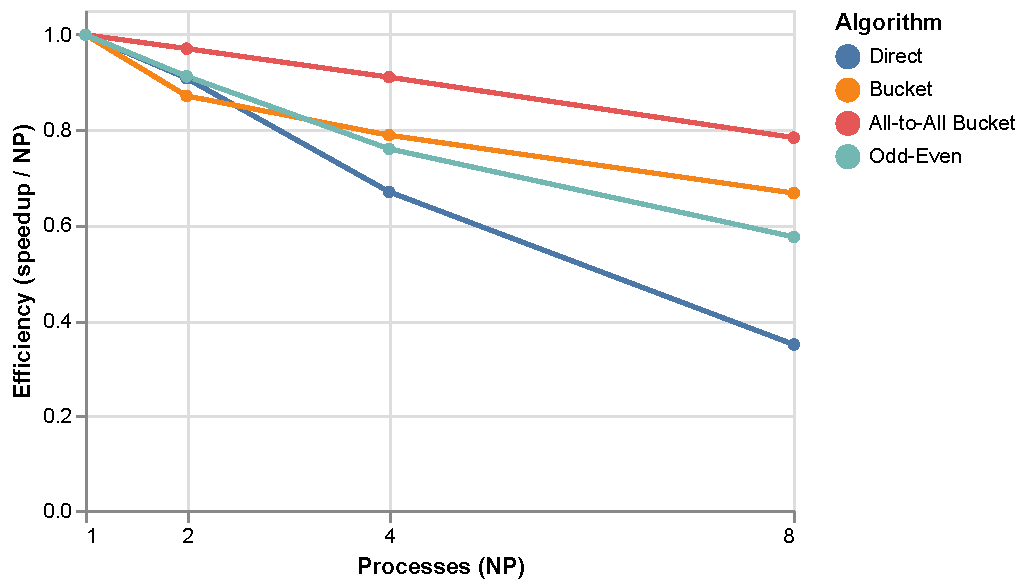
\includegraphics[width=\linewidth]{comparison-efficiency.pdf}
  \captionof{figure}{Parallel efficiency (speedup divided by NP).}
  \label{fig:comparison-efficiency}
\end{minipage}
\hfill
\begin{minipage}[c]{0.45\linewidth}
  \centering
  \small
  \setlength{\tabcolsep}{3pt}
  \begin{tabular}{rrrrr}
  \toprule
  NP & Direct & Bucket & All-to-All Bucket & Odd-Even \\
  \midrule
  1 & 1.00 & 1.00 & 1.00 & 1.00 \\
  2 & 0.91 & 0.87 & 0.97 & 0.91 \\
  4 & 0.67 & 0.79 & 0.91 & 0.76 \\
  8 & 0.35 & 0.67 & 0.78 & 0.58 \\
  \bottomrule
\end{tabular}

  \captionof{table}{Parallel efficiency.}
  \label{tab:comparison-efficiency}
\end{minipage}
